\documentclass[tikz,border=10pt]{standalone}
% Scale s = 0.011713 cm/px, centre (394.5, 255.5) px, y flipped
\begin{document}
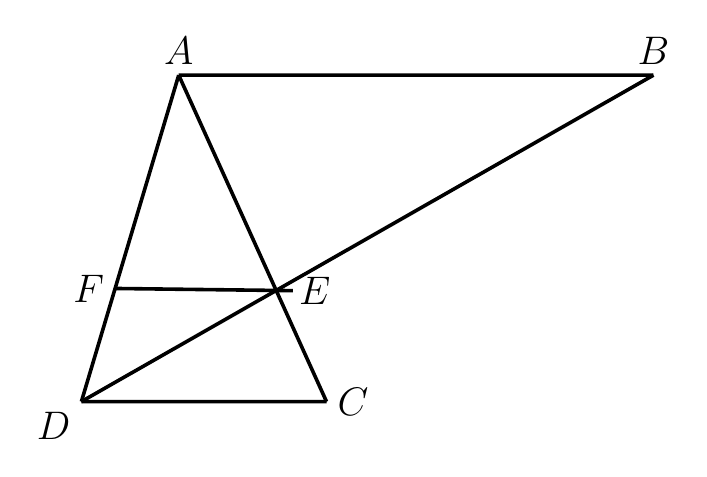
\begin{tikzpicture}[line width=1.3pt, line join=round]
  % Named coordinates (converted from pixels)
  \coordinate (A) at (-2.3933370193445036,2.0930320228852257);
  \coordinate (B) at (3.6355310201959385,2.092597574127436);
  \coordinate (C) at (-0.5162751164775709,-2.0529471936982953);
  \coordinate (D) at (-3.629260665765371,-2.0527228675567986);
  \coordinate (E) at (-1.1554525570224683,-0.6411576410145565);
  \coordinate (F) at (-3.2009633827739803,-0.6160519529201003);
  \coordinate (G) at (-0.9442422788120426,-0.6437499418229113); % FE extended to x=314 px

  % Solid segments
  \draw (A) -- (B);   % top AB
  \draw (D) -- (C);   % bottom DC
  \draw (A) -- (D);   % left leg AD (through F)
  \draw (B) -- (D);   % diagonal BD
  \draw (A) -- (C);   % diagonal AC
  \draw (F) -- (G);   % segment FE extended

  % Labels (outside the figure)
  \node[above] at (A) {\fontsize{13.5}{16.2}\selectfont $A$};
  \node[above] at (B) {\fontsize{13.5}{16.2}\selectfont $B$};
  % C: anchor west, level with vertex, just right of it
  \node[anchor=west] at (C) {\fontsize{13.5}{16.2}\selectfont $C$};
  \node[below left] at (D) {\fontsize{13.5}{16.2}\selectfont $D$};
  % E: anchor west, level with vertex; small xshift clears the FE stub end at x=314 px
  \node[anchor=west, xshift=0.15cm] at (E) {\fontsize{13.5}{16.2}\selectfont $E$};
  \node[left] at (F) {\fontsize{13.5}{16.2}\selectfont $F$};
\end{tikzpicture}
\end{document}
% GEOAGENT_REPAIR_V1 c18a466396f54661 175252e1cbb8135225ec6780dde6af52110705a08282fa37d5ba42795fb51bbf
